%%%%%%%% ICML 2020 SUBMISSION FILE %%%%%%%%%%%%%%%%%

\documentclass{article}

% Recommended, but optional, packages for figures and better typesetting:
\usepackage{microtype}
\usepackage{graphicx}
\usepackage{subfigure}
\usepackage{booktabs} % for professional tables

%%%%%%%%%%%%%%%%%%%%%%%%%%%%%%%%%%%%%%%%%%%%%%%%%%%%%%%%%%%%%%%%%%%%%%%%
% Mathematics
%%%%%%%%%%%%%%%%%%%%%%%%%%%%%%%%%%%%%%%%%%%%%%%%%%%%%%%%%%%%%%%%%%%%%%%%
\usepackage{amsmath}
\usepackage{bm}      % for bold greek letters
\usepackage{amssymb} % more math symbols
\usepackage{amsthm}
\usepackage{bbm}  % blackboard 1

% hyperref makes hyperlinks in the resulting PDF.
% If your build breaks (sometimes temporarily if a hyperlink spans a page)
% please comment out the following usepackage line and replace
% \usepackage{icml2020} with \usepackage[nohyperref]{icml2020} above.
\usepackage{hyperref}

% Attempt to make hyperref and algorithmic work together better:
\newcommand{\theHalgorithm}{\arabic{algorithm}}

% Use the following line for the initial blind version submitted for review:
\usepackage{icml2020}

% If accepted, instead use the following line for the camera-ready submission:
%\usepackage[accepted]{icml2020}

% The \icmltitle you define below is probably too long as a header.
% Therefore, a short form for the running title is supplied here:
\icmltitlerunning{Imputation Strategies with Signature Models}

\renewcommand{\subsubsection}[1]{\textbf{#1}

} % newlines are deliberate
\DeclareMathOperator*{\argmax}{arg\,max}
\DeclareMathOperator*{\argmin}{arg\,min}
\DeclareMathOperator*{\E}{\mathbb{E}}
\newcommand{\reals}{\mathbb{R}}
\newcommand{\naturals}{\mathbb{N}}
\newcommand{\sig}{\mathrm{Sig}^N}
\newcommand{\dataspace}{\mathcal{X}}
\newcommand{\lspace}{\mathcal{Y}}
\newcommand{\seriesspace}{\mathcal{S}}
\newtheorem{theorem}{Theorem}

\begin{document}

\twocolumn[
\icmltitle{Imputation Strategies with Signature Models for Irregularly Sampled Partially Observed Multivariate Time Series}

% It is OKAY to include author information, even for blind
% submissions: the style file will automatically remove it for you
% unless you've provided the [accepted] option to the icml2020
% package.

% List of affiliations: The first argument should be a (short)
% identifier you will use later to specify author affiliations
% Academic affiliations should list Department, University, City, Region, Country
% Industry affiliations should list Company, City, Region, Country

% You can specify symbols, otherwise they are numbered in order.
% Ideally, you should not use this facility. Affiliations will be numbered
% in order of appearance and this is the preferred way.
\icmlsetsymbol{equal}{*}

\begin{icmlauthorlist}
\icmlauthor{Michael Moor}{equal,ethz}
\icmlauthor{Patrick Kidger}{equal,oxford}
\icmlauthor{Max Horn}{ethz}
\icmlauthor{Christian Bock}{ethz}
\icmlauthor{Bastian Rieck}{ethz}
\icmlauthor{Karsten Borgwardt}{ethz}
\end{icmlauthorlist}

\icmlaffiliation{ethz}{Department of Biosystems Science and
Engineering, ETH Zurich, Switzerland}
\icmlaffiliation{oxford}{Mathematical Institute, University of Oxford, Oxford, United Kingdom}

\icmlcorrespondingauthor{Michael Moor}{michael.moor@bsse.ethz.ch}

% You may provide any keywords that you
% find helpful for describing your paper; these are used to populate
% the "keywords" metadata in the PDF but will not be shown in the document
\icmlkeywords{Machine Learning, ICML, signature, imputation, irregularly sampled, partially observed, multivariate, time series}

\vskip 0.3in
]

% this must go after the closing bracket ] following \twocolumn[ ...

% This command actually creates the footnote in the first column
% listing the affiliations and the copyright notice.
% The command takes one argument, which is text to display at the start of the footnote.
% The \icmlEqualContribution command is standard text for equal contribution.
% Remove it (just {}) if you do not need this facility.

\printAffiliationsAndNotice{\icmlEqualContribution} % otherwise use the standard text.

\begin{abstract}
The signature transform is a powerful transform, acting as a `universal nonlinearity' on the space of continuous vector-valued paths, and has recently received attention for use in machine learning. However real-world data is typically discretized, and must first be transformed into a continuous path before signature techniques can be applied. Existing solutions have often been ad-hoc and exhibit a variety of subtle flaws. In our analysis, we regard this as an imputation problem, study the merits of different schemes, evaluate them in theoretical terms and in terms of time series classification performance, and conclude by recommending particular novel and existing schemes.
\end{abstract}

\section{Introduction}\label{intro}
Originally described in \citep{Chen54, Chen57, Chen58} and popularised in the theory of rough paths and controlled differential equations \citep{lyons1998differential, hambly2010uniqueness, lyons2014rough}, the \emph{signature transform}, also known as the \emph{path signature} or simply \emph{signature}, consumes a continuous vector-valued path of bounded variation, and returns a graded sequence of statistics, which determine the path up to a negligible equivalence class.

Strikingly, every continuous function of a path can be recovered by applying a linear transform to this collection of statistics \citep[Proposition A.6]{kidger2019deep}. This `universal nonlinearity' property makes the signature a promising nonparametric feature extractor.

\subsubsection{Difficulties in applications}

Given the similarities between continuous paths and multivariate time series, it is natural to hope that we can use the tools that apply to one, namely the signature transform, and apply it to the other.

Of course, multivariate time series are not paths. For signature techniques to be applied, a continuous path must first be constructed from this data.

This should sound sensible: the data is often assumed to be a discretization of an underlying continuous process, and we now simply wish to recover some approximation to that process. Whilst methods such as e.g. recurrent neural networks may paper over the issue (see also our remarks later), signature methods require a path to be constructed.

We identify the task of going from a finite number of points to a continuous path in data space as an imputation problem; admittedly an unusual one, given the desire to impute an infinite number of values.

\subsubsection{The task at hand}

This certainly sounds like a simple enough goal. Indeed, every previous author considering practical uses of the signature transform has in some sense already solved it, one way or another. However, the seeming simplicity of the problem belies the subtle issues that can arise from it. Typical solutions are often ad-hoc, and tend to exhibit two particular flaws: non-causality, and a fragile dependence on sampling times in unrelated channels.
% TODO: more of a call to arms here

We believe this issue has gone unobserved due to the (perfectly sensible) behaviour of current software packages for computing the signature transform \citep{esig, iisignature, signatory}. Such packages typically compute the signature of a continuous piecewise linear path, which they expect to be described as a sequence of points, representing the knots between which the linear pieces interpolate.

This resembles a fully-observed sequence of data as might be encountered in practice. In this way the signature transform is sometimes held to operate on a sequence of data, rather than on a path, and it is precisely here that the opportunity for mistakes creep in.% In particular, what may seem like a causal imputation scheme with conventional techniques will fail to be so when signature techniques are applied.

Thus, we believe there is a need for a canonical solution to this problem.

\subsubsection{Contributions}

To the best of our knowledge, the identification that this is an issue at all is itself novel.

We analyze typical solutions to this problem and identify two key flaws.

We then demonstrate how these may be fixed. We propose a `meta-strategy', specific to the context of using signatures, which is capable of making certain existing imputation strategies robust against the two identified flaws; we term this \emph{causal signature imputation}. We then go onto propose a different strategy based on the Gaussian process adapter framework.

We justify our findings with both theoretical concerns and experimental results on time series classification tasks.

We conclude with some recommendations for practitioners. Depending on the nature of the problem we recommend either one existing (implicit) strategy, or one of our two proposed strategies.

Our code is available at (redacted for anonymity; see supplementary materials).
% TODO: Fill in with the actual link for the actual submission!

\subsubsection{Application beyond signatures}

Whilst the task of converting observed data into a path in data space is particularly important for signatures, we remark that it also arises in the context of, for example, convolutional and recurrent neural networks.

Convolutions are often thought of in terms of discrete sums, but they are perhaps more naturally described as the integral cross-correlation between the underlying data path $f$ and the learnt filter $g_\theta$. Given sample points $t_1, \ldots, t_n \in [0, T]$, this integral is then approximated via numerical quadrature:
\begin{equation*}
    \frac{1}{T}\int_0^T f(t) g_\theta(t) \mathrm{d}t \approx \frac{1}{n}\sum_{i = 1}^n f(t_i) g_\theta(t_i),
\end{equation*}
although we remark that the $1/n$ scaling is really only justified in the case that the $t_i$ are equally spaced.\footnote{The $g_\theta$ is typically a step function in `normal' convolutional layers. Some works exists on replacing it with e.g. B-splines \cite{TODO} to better handle irregular data. The oddity of scaling by $1/n$ with irregular data has not been explicitly addressed in the literature, at least to our knowledge; indeed quite conversely we have seen it used without remark.} Thus we see that with convolutions, we are implicitly interpreting the observed data as a path in data space.

Similarly, the connection between dynamical systems and recurrent neural networks are well known \citep{TODO, TODO, TODO}, and these tend to use a similar setup.

For non-signature methods as for signature methods, this implicit usage of data as a path in data space often seems to be swept under the rug, and we suspect it is one deserving further attention. However our focus here is specifically on solutions appropriate for signatures, and this larger problem is not one that we will explore further in this paper.

\section{Related work}
The general problem of imputing data is well-known and well-studied, and we will not attempt to describe it here; see for example \citep[Chapter 25]{gelman2007dataanalysis}. Common imputation schemes are to impute missing values as the mean of its channel, or to forward fill the last observed value. These methods typically only fill in missing discrete data points, and do not attempt to impute the underlying continuous path.

One approach that does impute a full continuous path is that of a \emph{Gaussian process adapter}, as in \citep{li2016scalable} and \citep{futoma2017mgp}. The data is modelled as coming from a Gaussian process. The posterior distribution, having observed the data, then gives continuous paths through data space. This has then allowed, for example, for uniformly resampling the data. Gaussian process adapters will be important to this study, although in our case they are of interest not because of uniform resampling, but because they provide a full continuous path.

% TODO: I reckon there's more that can be said here

A key motivation for this work is the use of the signature transform in machine learning. See for example \citep{primer2016, yang2016rotation, kiraly2016kernels, li2017lpsnet, yang2017leveraging, chevyrev2018signature, toth2019gp, fermanian2019embedding, morrill2019sepsis}, where the signature transform is typically used as a nonparametric feature extractor, on top of which a model (often linear or recurrent) is learnt. Some recent work has also investigated more tightly integrating the signature transform with machine learning frameworks; \citet{jeremythesis}, \citet{logsigrnn} and \citet{kidger2019deep} demonstrate how to use the signature transform\footnote{And the related logsignature transform; the difference between them will not be important for us.} within typical neural network models.

\citet[Appendix A]{kidger2019deep} give an approachable presentation on how signatures may be defined for piecewise linear paths. \citet{iisignature} and \citet{signatory} demonstrate efficient algorithms for computing the signature on piecewise linear paths.% We do not know of any explicit discussion on the necessity of the piecewise linearity for the purposes of computation; this appears to be `insider knowledge' so far without a published reference.

We do not know of any previous discussions specifically about the choice of imputation strategy. \citet{fermanian2019embedding} comes closest, by discussing the effect of different path-space transformations on empirical final results. In applications, one typically finds a sentence to the effect of: \emph{We impute missing data by forward filling ...}, without any discussion on the (unfortunate) implications of this.

\section{Theory}
We begin by fixing some notation and introducing a minimum amount of theory.

\begin{figure*}
	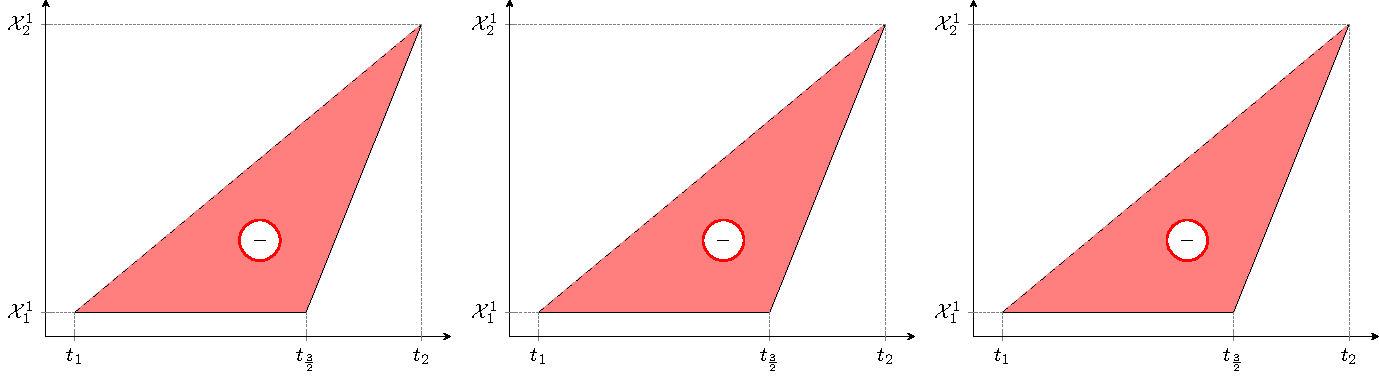
\includegraphics[width=\linewidth]{figures/sig_path.pdf}
	\label{fig:sig_path}
	\caption{First Figure}
\end{figure*}

\subsection{Path signatures}
Given a continuous, piecewise differentiable path $f \colon [a, b] \to \reals^d$, the \emph{signature transform up to depth $N$} may be defined by
\begin{equation*}
    \sig(f)=\left(\left(s_{i_1, \ldots, i_k}\right)_{1 \leq i_{1}, \ldots, i_{k} \leq d}\right)_{1 \leq k \leq N},
\end{equation*}
where each $s_{i_1, \ldots, i_k} \in \reals$ is defined by
\begin{equation}\label{eq:signature}
    s_{i_1, \ldots, i_k} = \underset{\,a<t_{1}<\cdots<t_{k}<b}{\int \cdots \int} \prod_{j=1}^{k} \frac{\mathrm{d} f_{i_{j}}}{\mathrm{d} t}\left(t_{j}\right) \mathrm{d} t_{1} \cdots \mathrm{d} t_{k}.
\end{equation}
This definition may straightforwardly be extended to paths of merely bounded variation by replacing these integrals with Stieltjes integrals with respect each $f_{i_j}$, and less straightforwardly extended further to paths of bounded $p$-variation by replacing them with rough integrals \citep{lyons1998differential}.

In brief, the signature transform may be interpreted as extracting information about order and area. One may interpret its terms as `the area/order of one channel with respect to some collection of other channels'.

For an exposition on the properties of the signature transform and its use in machine learning, we recommend either \citep{primer2016} or \citep[Appendix A]{kidger2019deep}. There is one fact that will prove important to our arguments later, however, so for completeness we repeat it here:
\begin{theorem}[Invariance to time reparameterisation]\label{theorem:invariancetime}
Let $f \colon [a, b] \to \reals^d$ be a continuous piecewise differentiable path. Let $\psi \colon [a, b] \to [c, d]$ be continuously differentiable, increasing, and surjective. Then $\sig(f) = \sig(f \circ \psi)$
\end{theorem}
In particular we see straight away that our choice of $a < b$ is unimportant: given some $c < d$ then we can choose any suitable $\psi \colon [a, b] \to [c, d]$, against which the signature will be invariant.

\subsubsection{Comparison to the Fourier and wavelet transforms}
The signature transform exhibits a certain similarity to the one-dimensional Fourier or wavelet transforms. Both are integral transforms operating on paths. However, in reality these transforms are fundamentally different. Both the Fourier and wavelet transforms are linear transforms, and operate on each channel of the input path separately. In doing so they model the path as a linear combination of elements from some basis.

Conversely, the signature transform is a nonlinear transform - indeed, it is a universal nonlinearity - and operates by combining information between different channels of the input path. In doing, the signature transform models \emph{functions of the path}; the universal nonlinearity property says that in some sense it provides a basis for such functions.

\subsubsection{Computing the signature transform}
Continuous piecewise linear paths are the paths of choice, computationally speaking, due to the fact that this is the only case for which efficient algorithms for computing the signature transform are known \citep{signatory}.

This is not a serious hurdle when one wishes to compute the signature of a path $f$ that is not piecewise linear -- as the signature of piecewise linear approximations to $f$ will tend towards the signature of $f$ as the quality of the approximation increases \citep{TODO} -- but it does enforce this requirement on our imputation schemes.

Thus all of the imputation schemes we examine will first seek to select a collection of points in data space (not necessarily only where we had data before), and then linear imputation will be performed to join them up into a piecewise linear path.

\subsection{Notation}
Given some set $A$, let the space of time series over $A$ be defined by
\begin{align*}
    \seriesspace(A) = \{((t_1, x_1), \ldots, (t_n, x_n)) \,\vert\, t_i \in \reals, x_i \in A,\qquad \\
    n \in \naturals, \text{ such that } t_1 \leq \cdots \leq t_n\}.
\end{align*}

Note the subtle point that the $t_i$ are separated by $\leq$, not $<$. We make this slight change because it will later prove important for one of our proposed imputation schemes. For example, contrast the corresponding definition in \citep[Section 1]{toth2019gp}.

Let $\lspace$ be a set and let $\dataspace_j$ be Banach spaces, typically $\reals$, for $j \in \{1, \ldots, d\}$ and $d \in \naturals$. Then we assume that we observe a dataset of labelled time series $(\mathbf{x}_k, y_k)$ for $k \in \{1, \ldots, N\}$, where $\mathbf{x}_k \in \seriesspace(\dataspace^*)$ and $y_k \in \lspace$, where $\dataspace^* = \prod_{j = 1}^d(\dataspace_j \cup \{*\})$ and $*$ represents no observation. We similarly define
$\dataspace = \prod_{j = 1}^d\dataspace_j.$ Thus $\dataspace$ is the data space, $\dataspace^*$ is the data space allowing missing data, and $\lspace$ is the set of labels.

\subsubsection{Terminology for imputation schemes}
% % TODO: check that we're consistent with 'data/path imputation'.
To avoid ambiguity, we will refer to standard imputation schemes, such as forward-fill, as a \emph{data-imputation} scheme, meaning to impute missing data points. In contrast we will use \emph{path-imputation} to describe the more general task of imputing the desired continuous path.

\subsection{Gaussian process adapter}\label{section:gpadapter}
Some (but not all) of the imputation schemes we consider are based on the uncertainty aware framework of multi-task Gaussian process adapters \citep{li2016scalable, futoma2017mgp}.

Let $\mathcal{W}, \mathcal{H}$ be some sets. Let $\ell \colon \lspace \times \lspace \to [0, \infty)$ be a loss function. Let $F \colon \dataspace^{[a, b]} \times \mathcal{W} \to \lspace$, be some (typically neural network) model, with $\mathcal{W}$ interpreted as a space of parameters. Let
\begin{align*}
\mu \colon [a, b] \times \seriesspace(\dataspace^*) \times \mathcal{H} &\to \dataspace\\
\Sigma \colon [a, b] \times [a, b] \times \seriesspace(\dataspace^*) \times \mathcal{H} &\to \dataspace    
\end{align*}
be mean and covariance functions, with $\mathcal{H}$ interpreted as a space of hyperparameters. The dependence on $\seriesspace(\dataspace^*)$ is to represent conditioning on observed values.

Then the goal is to solve
\begin{equation}\label{eq:gp-mc}
\argmin_{\mathbf{w} \in \mathcal{W},\bm{\eta} \in \mathcal{H}} \sum_{k=1}^N \overbrace{\rule{0pt}{0.5cm} \mathbb{E}_{\mathbf{z}_k \sim \mathcal{N}\left( \mu(\cdot, \mathbf{x}_k, \eta), \Sigma(\cdot, \cdot, \mathbf{x}_k, \eta)\right) } \big[ \ell(F(\mathbf{z}_k, \mathbf{w}), y_k) \big] }^{\text{$E_k$}} 
\end{equation}

As this expectation is typically not tractable, then it is estimated by Monte Carlo (MC) sampling with $S$ samples:
\begin{equation*}
E_k \approx \frac{1}{S} \sum_{s=1}^{S} \ell(F(\mathbf{z}_{s, k}, \mathbf{w}), y_k),
\end{equation*}
where
\begin{equation*}
    \mathbf{z}_{s, k} \sim \mathcal{N}\left( \mu(\,\cdot\,, \mathbf{x}_k, \eta), \Sigma(\,\cdot\,, \,\cdot\,, \mathbf{x}_k, \eta)\right).
\end{equation*}

Alternatively, one may forgo allowing the uncertainty to propagate through $F$ by instead passing the posterior mean directly to $F$; this corresponds to solving
\begin{align}\label{eq:gp-mean}
\argmin_{\mathbf{w} \in \mathcal{W},\bm{\eta} \in \mathcal{H}} \sum_{k=1}^N \ell(F(\mu(\,\cdot\,,\mathbf{x}_k, \eta), \mathbf{w}), y_k)
\end{align}

\section{Imputation}
%For simplicity of presentation, we will now assume that $\dataspace_j = \reals$.%, although in principle the theory actually only requires that $\dataspace_j$ is a Banach space.

Our end goal is to learn a function from $\seriesspace(\dataspace^*)$ to $\lspace$. Our belief (perhaps merely motivated by signature theory, but in this paper explicitly because we explicitly wish to apply signatures), is that this is sensibly done by selecting an path-imputation strategy
\begin{equation*}
    \phi \colon \seriesspace(\dataspace^*) \to (\reals \times \dataspace)^{[a, b]},
\end{equation*}
and only afterwards learning a map from $\dataspace^{[a, b]}$ to $\lspace$.

Explicitly, we seek $\phi$ such that
\begin{equation}\label{eq:phi}
\phi(\mathbf{x}) = f,    
\end{equation}
where
\begin{equation*}
\mathbf{x} = ((t_1, x_1), \ldots, (t_n, x_n)) \in \seriesspace(\dataspace^*),    
\end{equation*}
with each
\begin{equation*}
    x_i = (x_i^1, \ldots, x_i^d) \in \dataspace^* = \prod_{j = 1}^d (\dataspace_j \cup \{*\}),
\end{equation*}
and $f \colon [a, b] \to \reals \times \dataspace$ is continuous, piecewise linear, and such that there exist points
\begin{equation}\label{eq:ss}
a = s_1 < s_2 < \cdots < s_n = b    
\end{equation}
with $f(s_i) = (t_i, z_i)$, with $z_i^j = x_i^j$ for all $x_i^j \neq *$. (And with no restraint on $z_i^j$ if $x_i^j = *$.) Furthermore we impose that $f$ must be monotonically nondecreasing in its $t$ output.

Two remarks on this problem formulation.

First, we emphasise that the time series does not necessarily have to irregularly sampled or partially observed, although this is the most general setting. Even with a regularly spaced and fully observed time series, we must still path-impute the rest of the continuous path at the values in between.

Second, note that we have explicitly \emph{not} formulated this as seeking an $f \colon [t_1, t_n] \to \reals \times \dataspace$ with $f(t_i) = (t_i, z_i)$ with $z_i^j = x_i^j$ for $x_i^j \neq *$, as might na{\"i}vely be assumed. This alternate formulation is essentially what is typically used, see for example the `time embedding' of \citet{fermanian2019embedding}. However the slight extra generality in our formulation will be precisely what is necessary to solve the flaws in existing schemes, that we are about to identify.

\subsection{Flaws in existing schemes}\label{section:flaws}
We move on to discussing the flaws of existing schemes.

\subsubsection{Fragile dependence on sampling in unrelated channels}
Na{\"i}vely applying standard data-imputation schemes will typically result in the imputed path exhibiting an undesired dependence on the observations. This can result in dramatic changes in the areas-against-time computed by the signature; potentially going so far as to change the sign of the result.

Suppose that we have observed the (very short) time series
\begin{equation}\label{eq:flaw1}
    \mathbf{x} = ((t_1, x_1^1, x_1^2), (t_2, x_2^1, *)) \in \seriesspace(\reals^2).
\end{equation}
Perhaps we now apply, say, forward fill data-imputation, to produce
\begin{equation*}
    ((t_1, x_1^1, x_1^2), (t_2, x_2^1, x_1^2)).
\end{equation*}
Finally we linearly path-impute to create the linear path
\begin{align*}
    f &\colon [t_1, t_2] \to \reals \times \reals^2\\
    f &\colon t \mapsto (t, x_1^1\frac{t_2 - t}{t_2 - t_1} + x_2^1\frac{t - t_1}{t_2 - t_1}, x_1^2),
\end{align*}
to which we may then apply the signature transform. The signature includes certain areas of the path \citep{iisignature,fermanian2019embedding}, and so in particular we will have computed the following area:
% TODO: INSERT PICTURE

Now suppose we include an additional observation at some time $t_{3/2} \in (t_1, t_2)$, so that our data is instead
\begin{equation}\label{eq:flaw2}
    \mathbf{x} = ((t_1, x_1^1, x_1^2), (t_{3/2}, *, x_{3/2}^2), (t_2, x_2^1, *)).
\end{equation}
Then the same procedure as before will produce the data
\begin{equation*}
    \mathbf{x} = ((t_1, x_1^1, x_1^2), (t_{3/2}, x_1^1, x_{3/2}^2), (t_2, x_2^1, x_{3/2}^2)),
\end{equation*}
and now our function $f$, and the corresponding area we have computed, look like:
% TODO: INSERT PICTURE.

In this example, our choice of function $f$ has had its values in the $j=1$ channel changed due to the presence of completely unrelated observations in the $j=2$ channel; in turn this has now affected its signature. The closer $t_{3/2}$ is taken close to $t_2$, the greater the disparity.

This simple example underscores the danger of `just forward-fill data-imputing'. Doing so has introduced an undesired dependency on the simple \emph{presence} of an observation in other channels, with the change in our imputed path being determined by the \emph{time} at which this other observation occurred.

Indeed, this example holds for essentially every data-imputation scheme. The only standard scheme that survives this flaw is the linear data-imputation scheme.

Extending our previous example, linear data-imputation would produce
\begin{align*}
    \mathbf{x} = (&(t_1, x_1^1, x_1^2),\\
    &(t_{3/2}, x_1^1 \frac{t_2 - t_{3/2}}{t_2 - t_1} + x_2^1 \frac{t_{3/2} - t_1}{t_2 - t_1}, x_{3/2}^2),\\
    &(t_2, x_2^1, *)).
\end{align*}
Note that there is still an unimputed piece of data in the $x_2^2$ slot; we will return to this in a moment. Concerning the piece of data that has been data-imputed in the $x_{3/2}^1$ slot, we see that it is precisely what we would have path-imputed the value at $t_{3/2}$ as being, once we have performed linear path-imputation to generate the full path.

However, for the unimputed piece of data in the $x_2^2$ slot, the problem is that there is no `next observation' in the $j=2$ channel with which to use. In general, we cannot uniformly apply the linear data-imputation scheme, and must choose another scheme.

In general, we can summarise this by saying that \emph{when used with the signature transform, any traditional data-imputation scheme will have a fragile dependence on unrelated observations}.

\subsubsection{Non-causality}
Once fully observed data has been acquired, either by observation or data-imputation, then our next operation is always to perform linear path-imputation.

However, linear path-imputation is explicitly non-causal.

Given some $(t_i, x_i)$ and $(t_{i+1}, x_{i + 1})$, then the interpolating function $f$, considered on the interval $(t_i, t_{i + 1})$, will already be moving toward $x_{i + 1}$ before that piece of data has arrived:
\begin{equation*}
    f(t) = x_{i} \frac{t_{i + 1} - t}{t_{i + 1} - t_i} + x_{i + 1} \frac{t - t_i}{t_{i + 1} - t_i}\text{ for }t \in (t_i, t_{i + 1}).
\end{equation*}

Non-causality is of course not always a concern, but we will see in the next section that the same strategy for overcoming the previous flaw will overcome this one too.

We can summarise this by saying that \emph{when used with the signature transform, any traditional data-imputation scheme will be non-causal}.


% TODO: Need to do a comparison of different imputation schemes against one another
\subsection{Causal signature imputation}
We have spoke so far about the limitations of traditional data-imputation schemes, and at first glance one may be forgiven for thinking that these are issues are unavoidable. 

However, it turns out that we need not be limited just to these traditional imputation schemes. The trick is to consider time not as a \emph{parameterization}, but as a \emph{channel}. Contrast the two possible formulations that were discussed for $\phi$ defined in equation \eqref{eq:phi}.\footnote{To be clear, using time as a channel is already a well-known trick in the signature literature that we do not take credit for inventing! See for example \citep[Definition A.3]{kidger2019deep}. But it is an unusual set-up when not using signatures, so we simply wish to emphasise its importance here -- and it is pleasing that something commonly used in the theory of signatures is also what allows us to overcome what we observe as their limitations.}

This leads to our novel `meta-imputation strategy', which we refer to as \emph{causal signature imputation}. It will turn any traditional causal data-imputation strategy (for example, feed-forward) into a causal path-imputation strategy for signatures; at the same time it will overcome the other serious limitation that we identify.

Suppose we have some $\mathbf{x} \in \seriesspace(\dataspace^*)$, and some data-imputation strategy $c \colon \seriesspace(\dataspace^*) \to \seriesspace(\dataspace)$ that is causal in the usual sense.

Next, given
\begin{align*}
    \mathbf{x} = ((t_1, x_1), \ldots, (t_n, x_n)) \in \seriesspace(\dataspace)
\end{align*}
we define the operation $\Phi \colon \seriesspace(\dataspace) \to \seriesspace(\dataspace)$ by
\begin{align}
    \Phi(\mathbf{x}) = (&(t_1, x_1), (t_2, x_1), (t_2, x_2),(t_3, x_2),\nonumber\\
    &\ldots,\nonumber\\
    &(t_i, x_i), (t_{i + 1}, x_i), (t_{i + 1}, x_{i + 1}), (t_{i + 2}, x_{i + 1}),\nonumber\\
    &\ldots,\nonumber\\
    &(t_{n - 1}, x_{n - 2}), (t_{n - 1}, x_{n - 1}), (t_n, x_{n - 1}),(t_n, x_n)).\label{eq:causalsig}
\end{align}
That is, first time is updated, and then the corresponding observation in data space is updated. This means that the change in data space occurs instantaneously.

For each $n \in \naturals$ (and given $a < b$), fix any $s_i^{(n)}$ for $i \in \{1, \ldots, n \}$ as in equation \eqref{eq:ss}. (We will see that the exact choice is unimportant in a moment.) Given
\begin{align*}
    \mathbf{x} = ((t_1, x_1), \ldots, (t_n, x_n)) \in \seriesspace(\dataspace),
\end{align*}
let $\psi \colon \seriesspace(\dataspace) \to (\reals \times \dataspace)^{[a, b]}$ be the unique continuous piecewise linear path such that $\psi(s_i^{(n)}) = (t_i, x_i)$. Note that this is just a slight generalisation of the linear path-imputation that has already been performed so far; we are simply no longer asking for additional assumptions of the form $s_i^{(n)} = t_i$.\footnote{As in the $\mathbf{\phi}_\theta$ of \citep{toth2019gp}, for example.}

Finally, we put this all together, and define the causal signature imputation strategy $\phi_c$ associated with $c$ to be
\begin{equation*}
\phi_c = \psi \circ \Phi \circ c,
\end{equation*}
which will be a map $\seriesspace(\dataspace^*) \to (\reals \times \dataspace)^{[a, b]}$.

Thus $\phi_c$ defines a family of path-imputation schemes, parameterized by a choice of data-imputation scheme.

Why does this work?

First, note that the choice of $s_i^{(n)}$ is unimportant in this definition. By Theorem \ref{theorem:invariancetime}, the signature transform of $\phi_c(\mathbf{x})$ is invariant to this choice.

Second, note that sometimes holding time is fixed is a valid choice, by the definition for $\seriesspace$ in equation \eqref{eq:seriesspace}. (And there should hopefully be no moral objection to our definition of $\seriesspace$, as holding time fixed essentially just corresponds to a jump discontinuity; not such a strange thing to have occur.)

Third, we claim that $\phi_c$ is immune to both of the flaws we describe in section \ref{section:flaws}. Consider first the flaw of dependence on sampling in unrelated channels.

For simplicity take $c$ to be the forward-fill data-imputation strategy. Consider against the $\mathbf{x}$ defined in expression \eqref{eq:flaw1}. This means that
\begin{equation}\label{eq:causal1}
    \phi_c(\mathbf{x}) = \psi(\;((t_1, x_1^1, x_1^2), (t_2, x_1^1, x_1^2), (t_2, x_2^1, x_1^2))\;).
\end{equation}
% \begin{align*}
%     &\phi_c(\mathbf{x})(s)\\
%     &= \psi(\Phi(c(\mathbf{x})))(s)\\
%     &=\psi(\Phi(\;((t_1, x_1^1, x_1^2), (t_2, x_2^1, C_2))\;))(s)\\
%     &=\psi(\;((t_1, x_1^1, x_1^2), (t_2, x_1^1, x_1^2), (t_2, x_2^1, C_2))\;)(s)\\
%     &= \begin{cases}
%     (t_1 \frac{s_2^{(3)}- s}{s_2^{(3)} - s_1^{(3)}} + t_2 \frac{s - s_1^{(3)}}{s_2^{(3)} - s_1^{(3)}}, x_1^1, x_1^2)\\
%     \hphantom{\hphantom{(t_2, }\,x_1^2 \frac{s_3^{(3)} - s}{s_3^{(3)} - s_2^{(3)}} + C_2 \frac{s - s_2^{(3)}}{s_3^{(3)} - s_2^{(3)}}) }\text{ for }s \in [s_1, s_2]\\
%     (t_2, x_1^1 \frac{s_3^{(3)} - s}{s_3^{(3)} - s_2^{(3)}} + x_2^1 \frac{s - s_2^{(3)}}{s_3^{(3)} - s_2^{(3)}},\\
%     \hphantom{(t_2, }\,x_1^2 \frac{s_3^{(3)} - s}{s_3^{(3)} - s_2^{(3)}} + C_2 \frac{s - s_2^{(3)}}{s_3^{(3)} - s_2^{(3)}}) \text{ for }s \in (s_2, s_3]
%     \end{cases}
% \end{align*}
Contrast adding in the extra observation at $t_{3/2}$ as in equation \eqref{eq:flaw2}. Then
\begin{align}
    &\phi_c(\mathbf{x})(s)\nonumber\\
    &=\psi(\;((t_1, x_1^1, x_1^2), (t_{3/2}, x_1^1, x_1^2), (t_{3/2}, x_1^1, x_{3/2}^2),\nonumber\\ &\hspace{3.1em}(t_2, x_1^1, x_{3/2}^2), (t_2, x_2^1, x_{3/2}^2))\;).\label{eq:causal2}
\end{align}

Evaluating each $\psi$ will then in each case give a path with three channels, corresponding to $t, x^1, x^2$. Then it is clear that the $(t, x^1)$ component of the path in equation \eqref{eq:causal1} is just a reparameterization of the path in equation \eqref{eq:causal2}, a difference which is irrelevant by Theorem \ref{theorem:invariancetime}. (And the $x^2$ component of the second path has been updated to use the new information $x_{3/2}^2$.) Thus the proposed scheme is robust to such issues. If $c$ is any other causal data-imputation strategy then much the same analysis can be performed.

Now consider the second potential flaw, of non-causality. The issue previously arose because of the non-causality of the linear path-imputation. We see from equation \eqref{eq:causalsig}, however, such changes only occur in data space while the time channel is frozen; conversely the time channel only updates with the value in the data space frozen. Provided that $c$ is also causal, then causality will, overall, have been preserved.

There are interesting comparisons to be made between causal signature imputation and certain operations in the signature literature. First is the \emph{lead-lag} transform \citep{primer2016}. With the lead-lag transform, the entire path is \emph{duplicated}, and then each side is alternately updated. In causal signature imputation however, the path is instead \emph{split} between $t$ and $(x^1, \ldots, x^n)$, and then each side is alternately updated.

Second is the comparison to the linear and rectilinear embedding strategies \citep{fermanian2019embedding}. We identify that $\psi \circ \Phi$ may be interpreted as a hybrid between the linear and rectilinear embeddings: it is rectilinear with respect to an ordering of $t$ and $(x^1, \ldots, x^n)$, and linear on $(x^1, \ldots, x^n)$.

\subsection{Gaussian process adapters}\label{section:ourgpadapter}
Non-causality is not necessarily a worrying flaw, especially when not operating in an online setting. As such, we go on to consider another promising, but non-causal, path-imputation method, by adapting the Gaussian process adapter described in section \ref{section:gpadapter}.

One major drawback with the formulations of \citet{li2016scalable} and \citet{futoma2017mgp}, as described in equation \eqref{eq:gp-mc}, is that approximating the expectation outside of the loss function with Monte Carlo sampling is expensive.

During prediction, they propose to overcome this issue by sacrificing the uncertainty in the loss function and to simply pass the posterior mean, as in \eqref{eq:gp-mean}.\footnote{Equations \eqref{eq:gp-mc} and \eqref{eq:gp-mean} are of course not in general equal, so the same procedure should be used for both training and test -- despite the opposite being described at the end of Section 3.1 of \citep{li2016scalable}.}

To address both points, we propose to instead also pass the posterior covariance of the Gaussian process to the classifier $F$. This saves the cost of Monte Carlo sampling whilst explicitly providing the classifier with $F$ with uncertainty information.

This corresponds to solving
\begin{equation}\label{eq:gp-moments}
\argmin_{\mathbf{w} \in \mathcal{W},\bm{\eta} \in \mathcal{H}} \sum_{k=1}^N \ell(F(\mu(\,\cdot\,,\mathbf{x}_k, \eta), \Sigma(\,\cdot\,,\,\cdot\,,\mathbf{x}_k, \eta), \mathbf{w}), y_k),
\end{equation}
where instead now
\begin{equation*}
    F \colon \dataspace^{[a, b]} \times \dataspace^{[a, b] \times [a, b]} \times \mathcal{W} \to \lspace.
\end{equation*}

Training this model is no harder than the formulation of \citet{li2016scalable}. Abusing notation by conflating the Gaussian process sample $\mathbf{z}$ with its finite dimensional distribution that is of interest, simply decompose $\mathbf{z} = \mu + R \xi$, with $xi$ a standard multivariate normal and $R$ such that $\Sigma = RR^T$. The derivatives of equation \eqref{eq:gp-moments} are now no harder to describe than they were before.

In our context of interest, when $F$ is a signature model, then it is now straightforward to compute the signature of the Gaussian process, simply by sampling many points to construct a piecewise linear approximation to the process. Technically speaking, the choice of kernel has nontrivial mathematical implications for this procedure: if a Mat{\'e}rn 1/2 kernel is chosen, then the resulting path is not of bounded variation and the definition of the signature transform given in equation \eqref{eq:signature} does not hold, and rough path theory \citep{lyons1998differential} must instead be invoked to define the signature transform.

This formulation, whilst lacking causality, is nonetheless robust to the issue of fragility with respect to observations in unrelated channels. The Gaussian process adapter operates globally on all observed data, and observations in unrelated channels are allowed to be uncorrelated. This framework is also naturally more powerful at modelling than the explicit parameter-free schemes discussed thus far.

\section{Experiments}
To calculate the signature transform, we used the Signatory package of \citet{signatory}.

% TODO

\section{Recommendations}
We finish with some recommendations, based on our findings.

Whether causality is a concern or not, then causal signature imputation is simple to implement and effective at correcting the identified issues. If one takes the point of view that the signature transform is defined on data (rather than paths), then all that is necessary is to pick one's favourite imputation scheme, apply it as usual, and then apply the $\Phi$ of equation \eqref{eq:phi} to the imputed data, before using it. In more complicated models such as those proposed by \citet{kidger2019deep}, we recommend precomposing $\Phi$ to every usage of the signature transform.

If causality is not a concern, then we also recommend the variation of a Gaussian process adapter proposed in section \ref{section:ourgpadapter}. The implementation of this is much less straightforward, however. It remains a reasonable compromise to use linear data-imputation, which is unique in avoiding the flaw of dependence on unrelated channels, whilst accepting that there may be slight inconsistencies at either end of a partially observed time series.

\section{Conclusion}
We have identified a previously unobserved issue with the use of the signature transform in machine learning. We have analyzed the cause of the issue, and proposed practical, novel, solutions. We have made `recommendations for the practioner' on avoiding these pitfalls in the usage of the signature transform.


% TODO: explain why we don't study e.g. neural network based models

\section{Experiments}

% TODO: remove
% \subsection{Controlled Missingness}
% - UEA dataset with subsampling (totally random versus label-conditioned)
% \subsection{Classifying irregular and incomplete time series}
% - physionet 2012 mortality prediction \\
% - mimic sepsis \\

% Current experimental setup: \\
% - 50 epochs \\
% - early stopping after 20 epochs of val loss non-decreasing \\
% - learning rate $0.01$ to $0.0001$ (log uniform) \\
% - weight decay $0.001$ (Adam W optimizer) \\


% \begin{table}[]
%     \centering
%     \begin{tabular}{lcc}
%     \toprule
%      \textbf{Method} & \textbf{Average Precision} & \textbf{AUROC} \\
%      \midrule
%      GP-SigPoM (proposed)  & 0.4668 & 0.8166 \\% 
%     GP-Sig Adapter   & 0.3957 & 0.7786  \\
%     \end{tabular}
%     \caption{Performances on the Physionet 2012 mortality prediction task based on clinical time series. For sake of clarity, to assess time series classifiers we restrict to time series input data.}
%     \label{tab: Result table}
% \end{table}

\bibliography{ref}
\bibliographystyle{icml2020}


%%%%%%%%%%%%%%%%%%%%%%%%%%%%%%%%%%%%%%%%%%%%%%%%%%%%%%%%%%%%%%%%%%%%%%%%%%%%%%%
%%%%%%%%%%%%%%%%%%%%%%%%%%%%%%%%%%%%%%%%%%%%%%%%%%%%%%%%%%%%%%%%%%%%%%%%%%%%%%%
% DELETE THIS PART. DO NOT PLACE CONTENT AFTER THE REFERENCES!
%%%%%%%%%%%%%%%%%%%%%%%%%%%%%%%%%%%%%%%%%%%%%%%%%%%%%%%%%%%%%%%%%%%%%%%%%%%%%%%
%%%%%%%%%%%%%%%%%%%%%%%%%%%%%%%%%%%%%%%%%%%%%%%%%%%%%%%%%%%%%%%%%%%%%%%%%%%%%%%
\appendix


\end{document}


% This document was modified from the file originally made available by
% Pat Langley and Andrea Danyluk for ICML-2K. This version was created
% by Iain Murray in 2018, and modified by Alexandre Bouchard in
% 2019 and 2020. Previous contributors include Dan Roy, Lise Getoor and Tobias
% Scheffer, which was slightly modified from the 2010 version by
% Thorsten Joachims & Johannes Fuernkranz, slightly modified from the
% 2009 version by Kiri Wagstaff and Sam Roweis's 2008 version, which is
% slightly modified from Prasad Tadepalli's 2007 version which is a
% lightly changed version of the previous year's version by Andrew
% Moore, which was in turn edited from those of Kristian Kersting and
% Codrina Lauth. Alex Smola contributed to the algorithmic style files.
% TODO

